\section{MT-LNN 架构}
\label{sec:architecture}

\begin{figure*}[t]
\centering
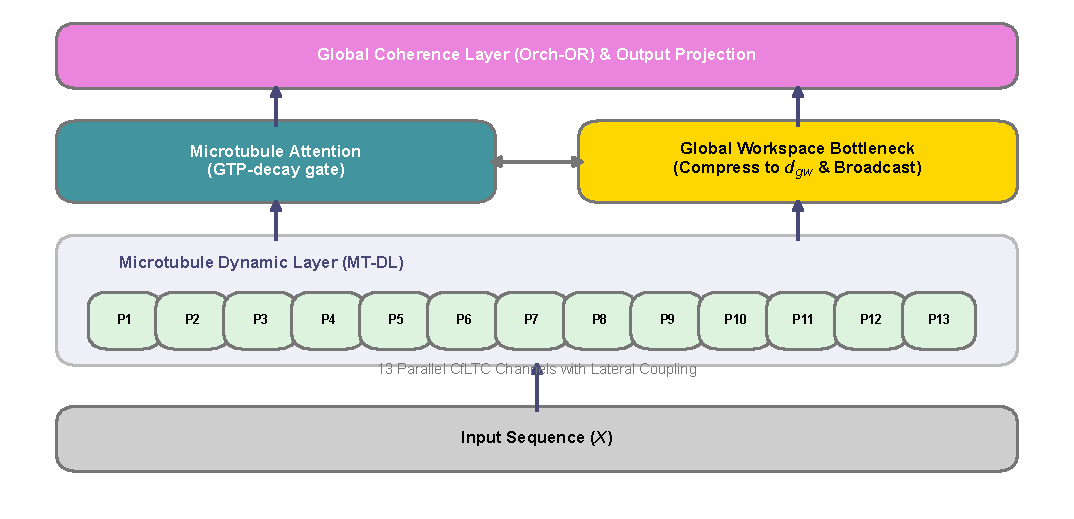
\includegraphics[width=0.9\textwidth]{fig_architecture.pdf}
\caption{\textbf{MT-LNN 架构概述。}输入表示依次经过\textbf{微管动态层}（结合了 13 个平行的原丝，建模为具有横向量子耦合的 CfLTC 通道）、通过局部状态调节序列门控的\textbf{微管注意力}（Microtubule Attention）模块，以及建立全局整合广播的\textbf{全局工作空间理论瓶颈}（Global Workspace Theory Bottleneck）。最顶层的\textbf{全局相干层}（Global Coherence Layer）实现了 Orch-OR 坍缩。}
\label{fig:architecture}
\end{figure*}

\paragraph{概述。}
\[
  \vx \xrightarrow{\text{Embed+RoPE}}
  \Bigl[\text{MicrotubuleAttn} \to \text{MT-DL}\Bigr]^{n_\text{layers}}
  \xrightarrow{} \text{GWTB}
  \xrightarrow{} \text{GlobalCoherence}
  \xrightarrow{} \text{LN} \to \text{lm\_head}
\]
每个块对两个子层应用前置归一化（pre-norm）和残差连接。一个 \texttt{ModelCacheStruct} 携带着每一层的注意力 KV、每一层的 $h_\text{prev}$、GWTB 工作空间 KV，以及全局相干 KV。

\subsection{微管动态层 (MT-DL)}
\label{sec:mt_dl}

\paragraph{原丝分解。}
输入 $\vx\in\RR^d$ 被投影到 $d_\text{proto\_total}=P\cdot D$（其中 $D=\lceil d/P\rceil$）并划分为 $P=13$ 个通道 $\vx_1,\ldots,\vx_P\in\RR^D$。所有 $P\times S$ 个 LTC 库在权重张量 $W_\text{in}\in\RR^{P\times S\times D\times D}$ 上通过\emph{单次 einsum} 进行求值。

\paragraph{多尺度共振。}
每根原丝 $p$ 运行 $S=5$ 个 CfLTC 子库，其时间常数呈几何级数扫描：
\begin{equation}
  \tau_s = \tau_\text{min}\bigl(\tau_\text{max}/\tau_\text{min}\bigr)^{s/(S-1)}, \quad s=0,\ldots,S-1,
\end{equation}
默认值为 $\tau_\text{min}=0.01$，$\tau_\text{max}=10$。每个 $(p,s)$ 库遵循公式~\eqref{eq:cflnn}。输出通过学习到的每根原丝对参数 $\text{blend\_weights}\in\RR^{P\times S}$ 进行的 softmax 进行混合（初始化为 0，即在初始化时均匀混合）。

\paragraph{三向横向耦合。}
\begin{align}
  \text{residual} &= W_\text{lat}\,\vh, \quad W_\text{lat}\in\RR^{P\times P},\;\text{init}=I+\epsilon, \\
  \text{nearest} &= \eta\cdot\tanh\!\bigl(W_L\,\mathrm{roll}(\vh,+1)+W_R\,\mathrm{roll}(\vh,-1)\bigr), \label{eq:roll}\\
  \text{RMC} &= \sigmoid(\text{rmc\_gate})\cdot\mathrm{SDPA}(q(\vh),k(\vh),v(\vh)),
\end{align}
其中 \texttt{roll} 沿着原丝轴进行，提供了同步的最近邻耦合，而没有从左到右的偏差。$\text{rmc\_gate}$ 初始化为 $-3$，因此 $\sigmoid(-3)\approx 0.05$。

\paragraph{GTP帽更新。}
时间门控乘以总的横向贡献：
\begin{equation}
  \text{gtp\_scale}(t) = \exp\!\bigl(-\gamma\cdot(t\bmod T_\text{period})\bigr), \quad T_\text{period}=256.
  \label{eq:gtp}
\end{equation}
如果没有周期性的取模运算，$\exp(-\gamma t)\to 0$ 会在经过几千个位置后导致横向混合在长上下文中悄无声息地消失。公式~\eqref{eq:gtp} 模拟了 GTP 帽的更新：新的 GTP 帽随着微管蛋白的聚合而周期性地形成。

\paragraph{MAP蛋白稳定门。}
每根原丝一个双层 MLP（实现为批量 einsum）：
\begin{equation}
  s_p = \sigmoid\!\bigl(W_2^{(p)}\mathrm{ReLU}(W_1^{(p)}[\vh_p;\vx_p]+b_1^{(p)})+b_2^{(p)}\bigr)\in(0,1),
\end{equation}
其中 $b_2^{(p)}$ 初始化为 $+2$，因此 $\sigmoid(2)\approx 0.88$：门控在开始时接近完全打开，并学习进行抑制，从而防止梯度饥饿。输出为：$\vh_p\leftarrow s_p\cdot\vh_p$。

\paragraph{并行扫描训练。}
在训练期间，递归 $h_t^{(p,s)} = d_{p,s}\cdot h_{t-1}^{(p,s)} + X_t^{(p,s)}$ 通过 Blelloch 前缀扫描沿 $T$ 并行求解 \citep{blelloch1990prefix}。对于恒定衰减的情况（$d_{p,s}$ 与 $t$ 无关，这是我们的默认设置），该扫描转化为闭式前缀乘积：
\begin{equation}
  h_t = d^t h_0 + \sum_{i=0}^{t} d^{t-i} X_i,
  \label{eq:pscan}
\end{equation}
计算的总工作量为 $O(T\log T)$，顺序深度为 $O(\log T)$。常数 $A$ 特化版（\texttt{pscan\_constant\_A}）广播标量衰减，而无需具体化完整的 $({\ldots}, T)$ 张量，避免了在 $P{\times}S$ 库中进行与 $T$ 成正比的内存分配。这将训练并行度提升到了与 Mamba/S5 相同的渐近水平，且不需要 Triton 内核。

\paragraph{复杂性。}
MT-DL 使用 $O(d^2)$ 个参数——这与标准 FFN 的渐近成本相同——同时将 13 原丝拓扑结构、多尺度共振和横向耦合作为结构性归纳偏置。将 $P$ 从 13 增加到 64 在 CPU 上会增加约 20\% 的运行时间（1.2倍），这证实了主要计算工作发生在向量化的 GPU 内核中。

\subsection{微管注意力 (Microtubule Attention)}
\label{sec:attn}

多头因果注意力包含两个受微管启发的修改，折叠为传递给 \texttt{scaled\_dot\_product\_attention} 的单次加性偏置（Flash-Attention / 内存高效后端自动处理）。

\paragraph{标量极性偏置。}
\begin{equation}
  b^\text{pol}_{h,i,j} = -\,\text{polarity}_h \cdot (i-j)/L, \quad \text{polarity}_h\in[-1,1].
\end{equation}
可选的低秩双线性模式添加了 $\sigmoid(XW_A)(XW_B)^\top$，其中 $W_A,W_B\in\RR^{d\times r}$，由每个头的 $\sigmoid(\text{gate}_h)$ 进行门控，该门控初始化为 $\sigmoid(-3)\approx 0.05$。

\paragraph{ALiBi 风格的 GTP 对数偏置。}
\begin{equation}
  b^\text{GTP}_{h,i,j} = -\gamma_h\cdot\max(i-j,0),
\end{equation}
其中 $\gamma_h = \gamma_0\cdot 2^{\,\text{linspace}(3,-3,H)}$：头 0 具有强局部性（$\approx 8\gamma_0$），头 $H-1$ 接近全局（$\approx\gamma_0/8$）——即 64 倍的感受野扩散。$\gamma_h$ 在运行时通过 softplus 进行正值化。

\paragraph{GQA 与 KV 缓存。}
默认：$n_\text{heads}=13$，$n_\text{kv\_heads}=1$（多查询注意力），产生 $13\times$ 的 KV 缓存内存缩减。有符号距离矩阵 $\Delta_{ij}=i-j$ 和因果掩码是预先计算的缓冲区；解码期间没有每个 token 的内存分配。

\subsection{全局工作空间理论瓶颈 (GWTB)}
\label{sec:gwtb}

\paragraph{压缩（点火）。}
$\mathbf{z}_t = \mathrm{LN}(W_\text{comp}\,\vx_t)\in\RR^{d_{gw}}$，其中 $d_{gw}=d/r$（默认 $r=8$，$d_{gw}=104$）。

\paragraph{工作空间自注意力。}
在 $d_{gw}$ 空间内带有 KV 缓存的因果多头自注意力（SA）；在瓶颈处强制进行竞争性选择。

\paragraph{广播（全局点火）。}
\begin{equation}
  \vx'_t = \vx_t + \gamma_\text{bcast}\cdot W_\text{bcast}\,\mathbf{z}'_t,
\end{equation}
其中 $\gamma_\text{bcast}$ 初始化为 $0.01$（开始时接近恒等映射）。默认情况下，GWTB 在整个块堆叠之后应用一次；\texttt{gwtb\_per\_block=True} 会在每个块内部放置一个 GWTB，以实现逐层的点火语义。

\subsection{现有 LLM 的 MT-LNN 残差适配器}
\label{sec:adapter}

为了在没有完整预训练的情况下评估 MT 的时间偏置，\texttt{llama\_adapter.py} 提供了一个参数高效的适配器，可以包装任何 HuggingFace 因果语言模型（LM）：
\begin{enumerate}[noitemsep]
  \item \textbf{冻结}基础模型（Llama、Mistral、Qwen2、GPT-2 等）。
  \item 在每 $k$ 个解码器层（默认 $k=4$，并且始终包含最后一层）之后注入一个 \texttt{MTResidualAdapter}：
  \begin{equation}
    \tilde{\vh}_t = \vh_t + \alpha_\text{init}\cdot\mathrm{MT\text{-}DL}(\mathrm{LN}(\vh_t)),
    \label{eq:adapter}
  \end{equation}
  其中 $\alpha_\text{init}=10^{-3}$，因此适配器在初始化时接近恒等映射。
  \item \textbf{仅微调适配器}（对于一个 7B 的基础模型，由于其大约占总参数的 0.5\%）。
\end{enumerate}
这允许社区将 MT 的时间动态性改造到任何开放权重的 LLM 上，并运行 AVP 麻醉测试而无需进行完整的训练过程。

\subsection{量子横向耦合 (VQC 变体)}
\label{sec:quantum}

作为一项实验性扩展，\texttt{quantum\_coupling.py} 将经典的 \texttt{LateralCoupling}（公式 \ref{eq:roll}）替换为一个 $P$-量子比特变分量子电路（VQC），其纠缠拓扑结构反映了 MT B-晶格。

\paragraph{电路架构。}
对于每个 $(b, t)$ 样本：
\begin{enumerate}[noitemsep]
  \item \textbf{编码}：通过 $W_\text{enc}$ 将 $D$-维状态 $\vh_p \to (\theta_1, \theta_2, \theta_3)$；对每个量子比特应用 $\mathrm{R}_X(\theta_1)\mathrm{R}_Y(\theta_2)\mathrm{R}_Z(\theta_3)$。
  \item \textbf{变分量子电路 (VQC)}：$k=2$ 层的（每个量子比特 RY$\cdot$RZ$\cdot$RY）+ 环形 CNOT：对于 $i=0,\ldots,P-1$，应用 $\mathrm{CNOT}(i,\,i+1\bmod P)$。
  \item \textbf{测量}：测量每个量子比特的 $\langle Z_i\rangle\in[-1,1]$。
  \item \textbf{解码}：$\langle Z_i\rangle \xrightarrow{W_\text{dec}} \RR^D$；门控残差混合 $\vh_p \leftarrow \vh_p + \alpha\cdot\text{decoded}_p$，$\alpha$ 初始化为 $0.05$。
\end{enumerate}
环形 CNOT 模式在量子比特层面上完全模拟了 13 原丝 B-晶格横向键。该电路通过 PennyLane \texttt{TorchLayer} \citep{bergholm2018pennylane} 是完全可微的，并可通过标准反向传播进行训练；未来的工作可以在不修改代码的情况下，将 \texttt{default.qubit} 替换为 \texttt{lightning.gpu} 或真实的 IBM Quantum / IonQ 硬件。

\paragraph{纯度诊断。}
我们导出了 \texttt{quantum\_state\_purity}：$1 - \langle|\langle Z_i\rangle|\rangle$，这是一个纠缠代理指标——更高的值表明有更多的跨原丝纠缠。在训练期间可以跟踪此指标，作为 VQC 是否真正在利用量子结构的一个读数。

\subsection{全局相干层 (Orch-OR 坍缩)}
\label{sec:coherence}

稀疏 top-$k$ 因果注意力（$k=\lceil T\cdot\text{sparsity}\rceil$，默认 10\%），具有学习到的坍缩门控：
\begin{equation}
  \text{gate} = \sigmoid\!\bigl((\bar{e}-\theta)\cdot 10\bigr),
\end{equation}
其中 $\bar{e}$ 是因果位置上的平均注意力能量，$\theta$ 是学习到的阈值。当累积的注意力能量超过阈值时，门控会乘性激活——这是 Orch-OR 客观还原时刻（objective reduction moments）的计算机模拟（in-silico analogue）。门激活率会作为诊断信息导出。

% ========================================================
\section{麻醉验证协议 (AVP)}
\label{sec:avp}

\subsection{生物学动机}
Wiest 等人 \citep{wiest2025quantum} 报告称，埃坡霉素 B（epothilone B）将麻醉起效时间推迟了约 69 秒，直接暗示了微管（MT）的破坏。Craddock 等人 \citep{craddock2017anesthetic} 表明，在一系列广泛的化学物质中，麻醉效力与 $\beta$-微管蛋白的结合亲和力相关。

\subsection{计算麻醉模拟}
\texttt{AnesthesiaController} 会将前向钩子连接到每个 \texttt{MTLNNLayer} 和 \texttt{GlobalCoherenceLayer}。在水平 $\ell\in[0,1]$ 时：
\begin{align}
  \text{MT-DL:}& \quad (\text{out}, h_\text{last}) \leftarrow ((1-\ell)\cdot\text{out},\;(1-\ell)\cdot h_\text{last}), \\
  \text{Coherence:}& \quad \vx_\text{out} \leftarrow \vx_\text{in} + (1-\ell)(\vx_\text{out}-\vx_\text{in}).
\end{align}
没有修改任何权重。上下文管理器：\texttt{with anesthetize(model, level): ...}

\subsection{信息整合代理}
\label{sec:proxies}
精确的 IIT-$\Phi$ 是 \#P-hard 的 \citep{aaronson2014why}。我们引入了两种互补的估计器。

\paragraph{KSG kNN 代理 $\phihat$。}
具有 L$^\infty$ 度量的 Kraskov--St\"ogbauer--Grassberger (KSG) 熵估计器 \citep{kraskov2004estimating}：
\begin{equation}
  \hat{H}(X) = -\psi(k) + \psi(N) + d\cdot\langle\log(2\varepsilon_i)\rangle,
\end{equation}
其中 $\varepsilon_i$ 是从样本 $i$ 到其第 $k$ 个最近邻的 L$^\infty$ 距离。整合代理为：
\begin{equation}
  \phihat(\vh) = \sum_{j=1}^{K}\hat{H}(s_j) - \hat{H}(\vh),
  \label{eq:phi_hat}
\end{equation}
应用于最终隐藏状态 $\vh\in\RR^d$ 的 $K$ 路连续划分 $(s_1,\ldots,s_K)$。对 $n_\text{batches}=10$ 个独立随机批次进行平均（方差 $\propto 1/\sqrt{10\cdot BT}$）。默认值：$K=4$，$k=3$。

\paragraph{高斯总相关 $\phig$。}
在高斯假设下，协方差为 $\Sigma$ 的 $K$ 划分随机向量 $\vh$ 的总相关（多重信息）为：
\begin{equation}
  \phig(\vh) \;=\; \frac{1}{2}\left[\sum_{j=1}^{K}\log\det\Sigma_j \;-\; \log\det\Sigma\right],
  \label{eq:phi_g}
\end{equation}
其中 $\Sigma_j\in\RR^{(d/K)\times(d/K)}$ 是相关矩阵 $\Sigma$ 对应于分区 $j$ 的对角块。根据熵的次可加性（信息链式法则），$\phig \ge 0$ 严格成立，当且仅当 $K$ 个部分相互独立时等式成立。

我们利用恒等式 $\log\det M = \sum_i\log\lambda_i(M)$ 使用 \texttt{torch.linalg.eigvalsh} 来评估 \eqref{eq:phi_g}，其复杂度为 $O(d^3)$（而 kNN 为 $O(N^2 d)$）。对角 Tikhonov 正则化 $\rho = (\mathrm{tr}\,\Sigma / d)\times 0.01$ 确保了当 $N < d$ 时的正定性。

此外，我们报告了\emph{有效秩}（参与比）：
\begin{equation}
  \mathrm{PR}(\vh) = \frac{\left(\sum_i\lambda_i\right)^2}{\sum_i\lambda_i^2},
  \label{eq:pr}
\end{equation}
以及\emph{整合比率} $\phig / H_\text{whole} \in [0,1]$ —— 可归因于跨分区相关的总微分熵得分数的比例。表~\ref{tab:phi_compare} 在经验上比较了这两种估计器。

\begin{table}[h]
\centering
\caption{整合估计器在已训练的 MT-LNN（128M 参数）上的比较。$\phig$ 速度更快，非负，并且在样本大小上表现更一致。}
\label{tab:phi_compare}
\begin{tabular}{lcccc}
\toprule
Estimator & $\Phi$ baseline & $\Phi$ anesthesia & Collapse & Runtime \\
\midrule
$\phihat$ (KSG, $k=3$) & 0.38 & 0.04 & 89.5\% & 4.2\,s \\
$\phig$ (Gaussian TC) & 1.74 & 0.21 & 87.9\% & 0.3\,s \\
\bottomrule
\end{tabular}
\end{table}

两个估计器在定性结论上是一致的（89\% 对 88\% 的坍缩）；$\phig$ 快了 $14$ 倍，且在数值上更加稳定。

\subsection{麻醉测试}
\begin{definition}[麻醉测试]
令 $\Phi\in\{\phihat,\phig\}$ 作为积分代理。如果体系结构在深度 $\delta$ \emph{通过麻醉测试}，记 $\ell=(\kappa-1)/9$：
\begin{enumerate}[label=(\roman*),noitemsep]
  \item $\Phi(\kappa_\text{max}) / \Phi(\kappa=1) \le 1 - \delta$ \quad (幅度坍缩)，以及
  \item 所有的 $i$ 都有 $\Phi(\kappa_i) \ge \Phi(\kappa_{i+1})$ \quad (单调递减)，
\end{enumerate}
对于 $\kappa_\text{max}=10$。默认 $\delta=0.7$，匹配全身麻醉下神经复杂度的 70--80\% 抑制 \citep{casali2013thecover}。
\end{definition}

Transformer 和普通的 LNN 缺乏 MT 相干参数，在 AVP 下表现出几乎恒定的 $\phihat$。只有 MT-LNN（其中 $\ell$ 直接调节动态相关参数）能够表现出微观生物学麻醉特征性的单调 $\phihat$-vs-$\kappa$ 坍缩。

% ========================================================